\documentclass[twoside,11pt]{article}

\usepackage{amssymb,amsmath,amsthm} 
\usepackage{geometry, graphicx}
\usepackage{tabulary}
\usepackage{upgreek}
\usepackage{siunitx}
\usepackage{caption}
\usepackage{subcaption}
\usepackage{csvsimple}
\usepackage{hanging}
\usepackage[export]{adjustbox}
\usepackage{multirow}

\usepackage{enumitem}

\usepackage{mathtools}

\DeclarePairedDelimiter\abs{\lvert}{\rvert}%
\DeclarePairedDelimiter\norm{\lVert}{\rVert}%

% Swap the definition of \abs* and \norm*, so that \abs
% and \norm resizes the size of the brackets, and the 
% starred version does not.
\makeatletter
\let\oldabs\abs
\def\abs{\@ifstar{\oldabs}{\oldabs*}}
%
\let\oldnorm\norm
\def\norm{\@ifstar{\oldnorm}{\oldnorm*}}
\makeatother

\usepackage{jmlr2e}
\usepackage{url}

% Definitions of handy macros can go here

\newcommand{\dataset}{{\cal D}}
\newcommand{\fracpartial}[2]{\frac{\partial #1}{\partial  #2}}


\graphicspath{ {../images} }    

% Heading arguments are {volume}{year}{pages}{submitted}{published}{author-full-names}


% Short headings should be running head and authors last names

\ShortHeadings{CMD of M15 Star Cluster}{Jardee}
\firstpageno{1}

\begin{document}

\title{CMD Characterization of the Messier 15 Star Cluster}

       
\author{\name William Jardee\email willjardee@gmail.com \AND
       	\name Sage McNutty \email  \AND 
        \name Charlie Sanders \email  \\
       	\addr Physics Major\\
       	Montana State University\\
       	Bozeman, MT 59715, USA
      	}
\editor{William Jardee}

\maketitle

\begin{abstract}%   <- trailing '%' for backward compatibility of .sty file
This paper reports the CMD of the M15 star cluster from unprocessed images collected from a SBIG Aluma 814 CCD camera. The methods used to process the images are briefly touched on. Images taken in red, green, and blue filters are processed with PSF photometry and crossmatched to create a CMD of the brightest stars along the edge of the cluster. The characteristics of the horizontal ``red giant branch" can be seen, and used to roughly verify the commonly accepted metallicity of the cluster. 
\end{abstract}

\begin{keywords}
CMD, M15, Prometheus
\end{keywords}

\section{Introduction and Background}
It is amazing how humans, being bound to our planet for all of our history, have been able to characterize and explore the stars in a way that is best described as intimate. By collecting data as simple as the brightness and color of stars, the age and composition of galaxies can be deduced. The primary method that is used to collect this data is through effectively visual descriptions of the data, called Color Magnitude Diagrams (CMDs). On a CMD, a distinctive color (usually either green or red) is plotted against the difference of two colors (usually blue and red). A theoretical model can then be fit onto the data using two primary tunable parameters: the age of the galaxy and the metallicity of the galaxy. With come clever manipulation, such as through taking into consideration the unknown parameters of the distance of the galaxy and the extinction rate of specific colors before they reach the telescope (from atmospheric scattering, for example), useful data can be drawn out of even mediocre data, as will be shown in this paper. 

A couple key characteristics of the age of a galaxy star cluster will be brought up, but not explained in any exhaustive detail to not delay the purpose of this report. In the life cycle of a star, in the beginning it is dense and hot. But, as time goes along the dense structure begins to ``puff out" so that is is less dense, cooler, and much brighter. This evolution takes longer time for more massive stars who have to burn through more matter to reach the same point in their lives. For this reason, more massive stars (often ones that are said to have more metals in them) will follow a much different trajectory then younger, lighter stars. On the standard evolution, there is a transfer where stars deviate into giants, often called the ``giant branch". This deviation shows up in much brighter stars and relates strongly with the metallicity of cluster. This will be important later, as more luminous stars are easier to detect, thus it is much easier to deduce how massive a cluster is than how old it is. 

The target of this analysis will be the Messier 15 (M15) globular star cluster. This star cluster was chosen because it has a couple key characteristics. Being one of the oldest cluster easily observable, the cluster is easy to see and has a very obvious horizontal branch. This horizontal branch should make analysis of the CMD much easier if the data turns out to be lack-luster. The cluster also has a prime viewing window, being at minimum airmass at around 10 in the evening over Bozeman, MT.\footnote{I won't labor the point of coordinates of Bozeman or the timezone because I know my audience will be very comfortable with the location.} 

\section{Data Collection}
The data collected to be analyzed fell victim to a couple key issues. The primary one was inexperience. The data was collected from a CCD camera that was still being ``played with" to understand all the features that could be used. One such example was the lack of accurate tracking. Since the tracking of the camera didn't seem to be very good, long exposures were avoided and will prevent the ability to see dimmer stars. A lot of time that could have been used during the ideal viewing time was also wasted, as the new users of the camera were attempting to understand all the parameters of the software before collecting data. These issues will show up a couple more times throughout the analysis and will be dealt with the best that can, but obviously will impact the final project.

\subsection{Equipment}
The telescope used was a Celestron 9.25'' EdgeHD f/10 with a SBIG Aluma 814 CCD camera. The color filters used were the Celestron LRGB Filter Set that came with the camera. The images were captured and recorded with the MaximDL program that was provided.

\subsection{Collection}
The science images were collected on the 9th of October 2021 at around 10:00 PM MST. Before dusk flat images were taken against the sky; however, the evening was particularly cloudy and good flat data was not able to be taken. These clouds were fought against for the whole night, but didn't get in the way of the science images. Other group's flat images were used to create a flat image for each of the filters to be used in analysis of the images. 70 bias images and 70 dark images were taken during the night to analyze the noise and dark current of the camera. A plethora of images were collected with the red, green, and blue filters provided on the camera.

Because of a lack of experience on the camera, the sky tracking was not working and consequently a lot the exposures taken exhibited smearing that left them unusable for a CMD. Luckily there were one image of each color that seemed to have low-enough noise that they could be analyzed. Because of an oversight during data collection, the option for overscan was not selected and the overscan regions given with the images were only a couple of pixels wide. Since this is not something that can be fixed in post, there is a little more noise than would be expected if the overscan were there. 

\section{Analytic Methods}
Most of the analysis that was done mirrored methods taught inclass and were then translated by David Nidever to a collection of packages [cite here]. There was one issue during registration and crossmatching between data-types were the package assumed a byte structure that was not naturally read in from the .fits data. Instead of doing a byte-reordering, a quick supplementary code was written to exploid the WCS objects from Astropy and interative searching to register and cross-match the three different color images; red, green, and blue. 

\subsection{Image Analysis}
\begin{figure}[ht]
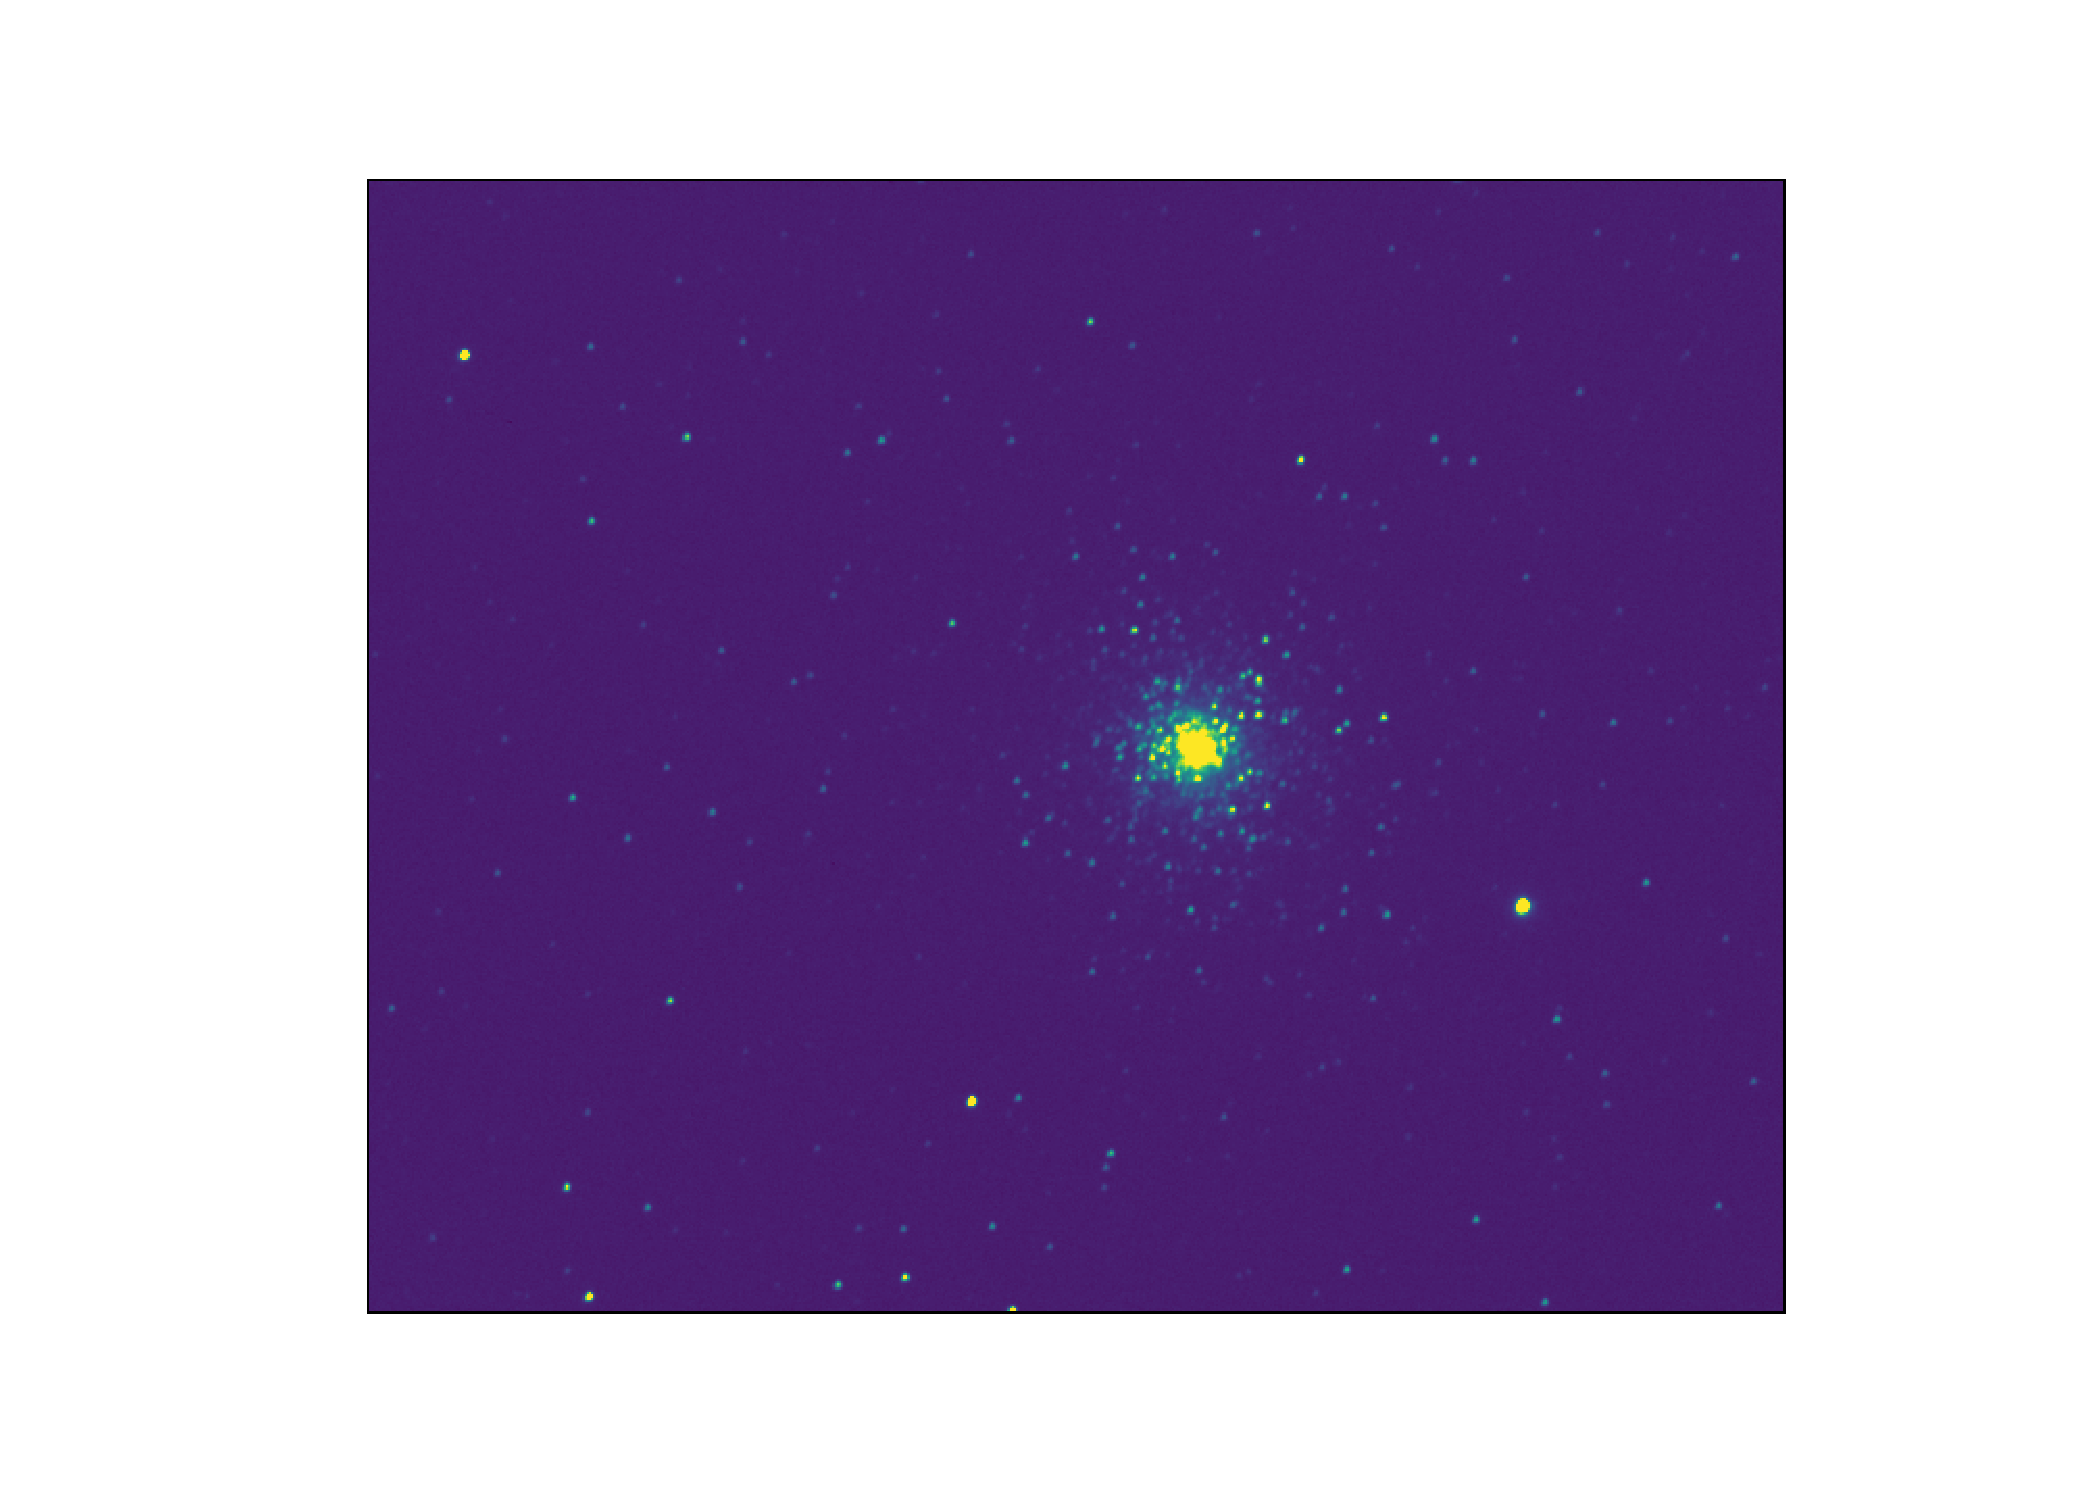
\includegraphics[width=\textwidth]{red_pic.pdf}
\caption{The best science image taken. The image is in the red filter and has already been fully processed.}
\label{fig:red}
\end{figure}

The 70 bias images, 70 dark images, and flat images were all processed to create a master-bias, master-dark, and master-flat image, respectively, using the Bozepy module. These three images were applied to all the science images taken, as well as overscan correcting and trimming, to allow for prime candidates to be picked. The best red, green and blue images were chosen, and the best of those three (the red) can be seen in Figure~\ref{fig:red}.

\subsection{Photometry}
\begin{figure}[ht]
\centering
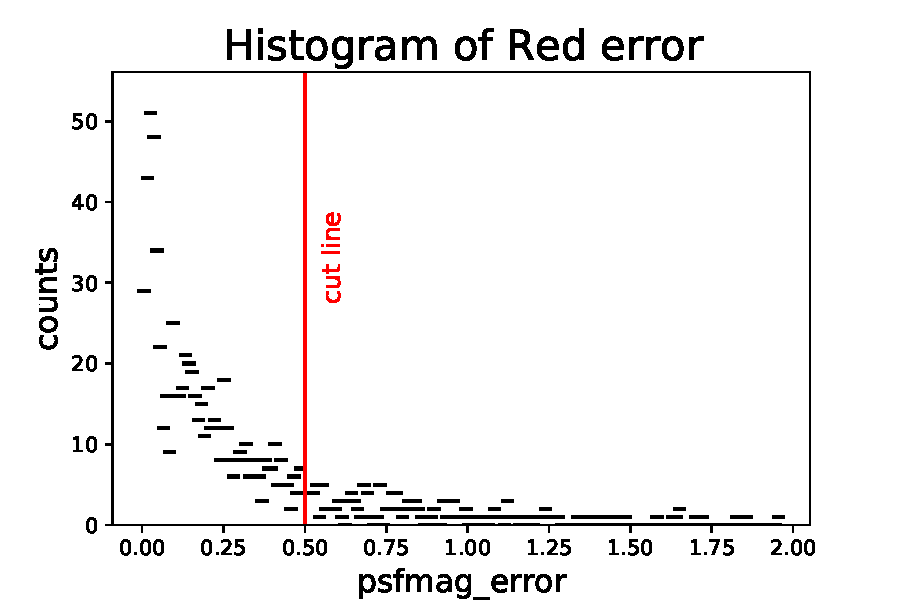
\includegraphics[scale=.75]{cutline.pdf}
\caption{The appropriate Error for the PSF photometry analysis. The error goes on till a very large magnitude, but the count seems to star leveling off around 1/2. Since it seems that most of the quality data has already been gathered at this point, everything to the right of the ``cut line" was removed from the analysis. This really cleaned up the data.}
\label{fig:cutline}
\end{figure}

The M15 star cluster is a globular cluster, meaning that the stars are very densely packed. Consequently, the footprint of each star in the images were overlapping and could not be distinguished using simple apeture photometry. Instead, PSF photometry was used to fit a penny model to the stars. The Penny model blends together a Gaussian fit and a Lorentzian fit to every star detected in the image. The Gaussian fit matches the primary distribution of the star and the Lorentizian accounts for the diffused characteristics, often called the ``wings" of the star. The number of stars that were found and analyzed can be found in Table~\ref{tab:counts}. As to be expected, the dense center of the cluster was difficult to distinquish stars from. However, it is interesting that many of the stars many of the stars that were found near the center were picked up by all three colors (Figure~\ref{fig:stars}). 

Considering how noisy the image was, there was some trimming that needed to happen to remove potential extra noise from this list of stars. This was justified by realizing that even if there were star of magnitude 50 detected, their characteristics could not be analyzed using simple CMD analysis. And there were multiple stars with magnitudes about 40. So, the histogram of the error can be seen in Figure~\ref{fig:cutline} and any stars that have error above the point where it begins to level out were cut. This meant that the only stars considered had a reasonable PSF fit (The number of remaining stars can be seen in Table~\ref{tab:counts}).

\subsection{Registration and Crossmatching}
Since the tracking on the telescope was not accurately working the night of the data collection, the reference locations for each image was inaccurate. Each of the images being analyzed there given to an online resource to locate key stars and provide a WCS coordinate file for each of the images [reference nova]. Using the reference star given by the online resource, the pixel location of that star was identified and all three WCS objects were aligned to the same object. Because of this, the stars found during the photometry step could all be translated into one pixel frame. The red image was chosen for this frame because it was the best looking image and allowed all the stars to be plotted against a good looking background. 

As can be seen in Figure~\ref{fig:stars}, not all the stars can be found in all three colors. Since the colors need to be compared, they had to be cross-matched so that all points had all three colors. This was cone by iterating through all the stars in one color and compared against all the stars in another color, searching for the closest pairing. The closest match for each star in the first list were save, at the end if multiple stars matched with the same star, the closest one was kept and the rest were discarded. A max radius was also implemented, removing any matches that were more than 20 pixels apart. All these stars were then compiled together, and stars that did not have all three colors were removed (Table~\ref{tab:counts}). 

All the numbers chosen were tuned until at least 400 stars were left over. The selection processed used was much more rigorous than that provided by the Prometheus module, but the number of data points provided by this analysis was ample enough to see the main characteristics in the CMD. 

\begin{figure}[ht]
\centering
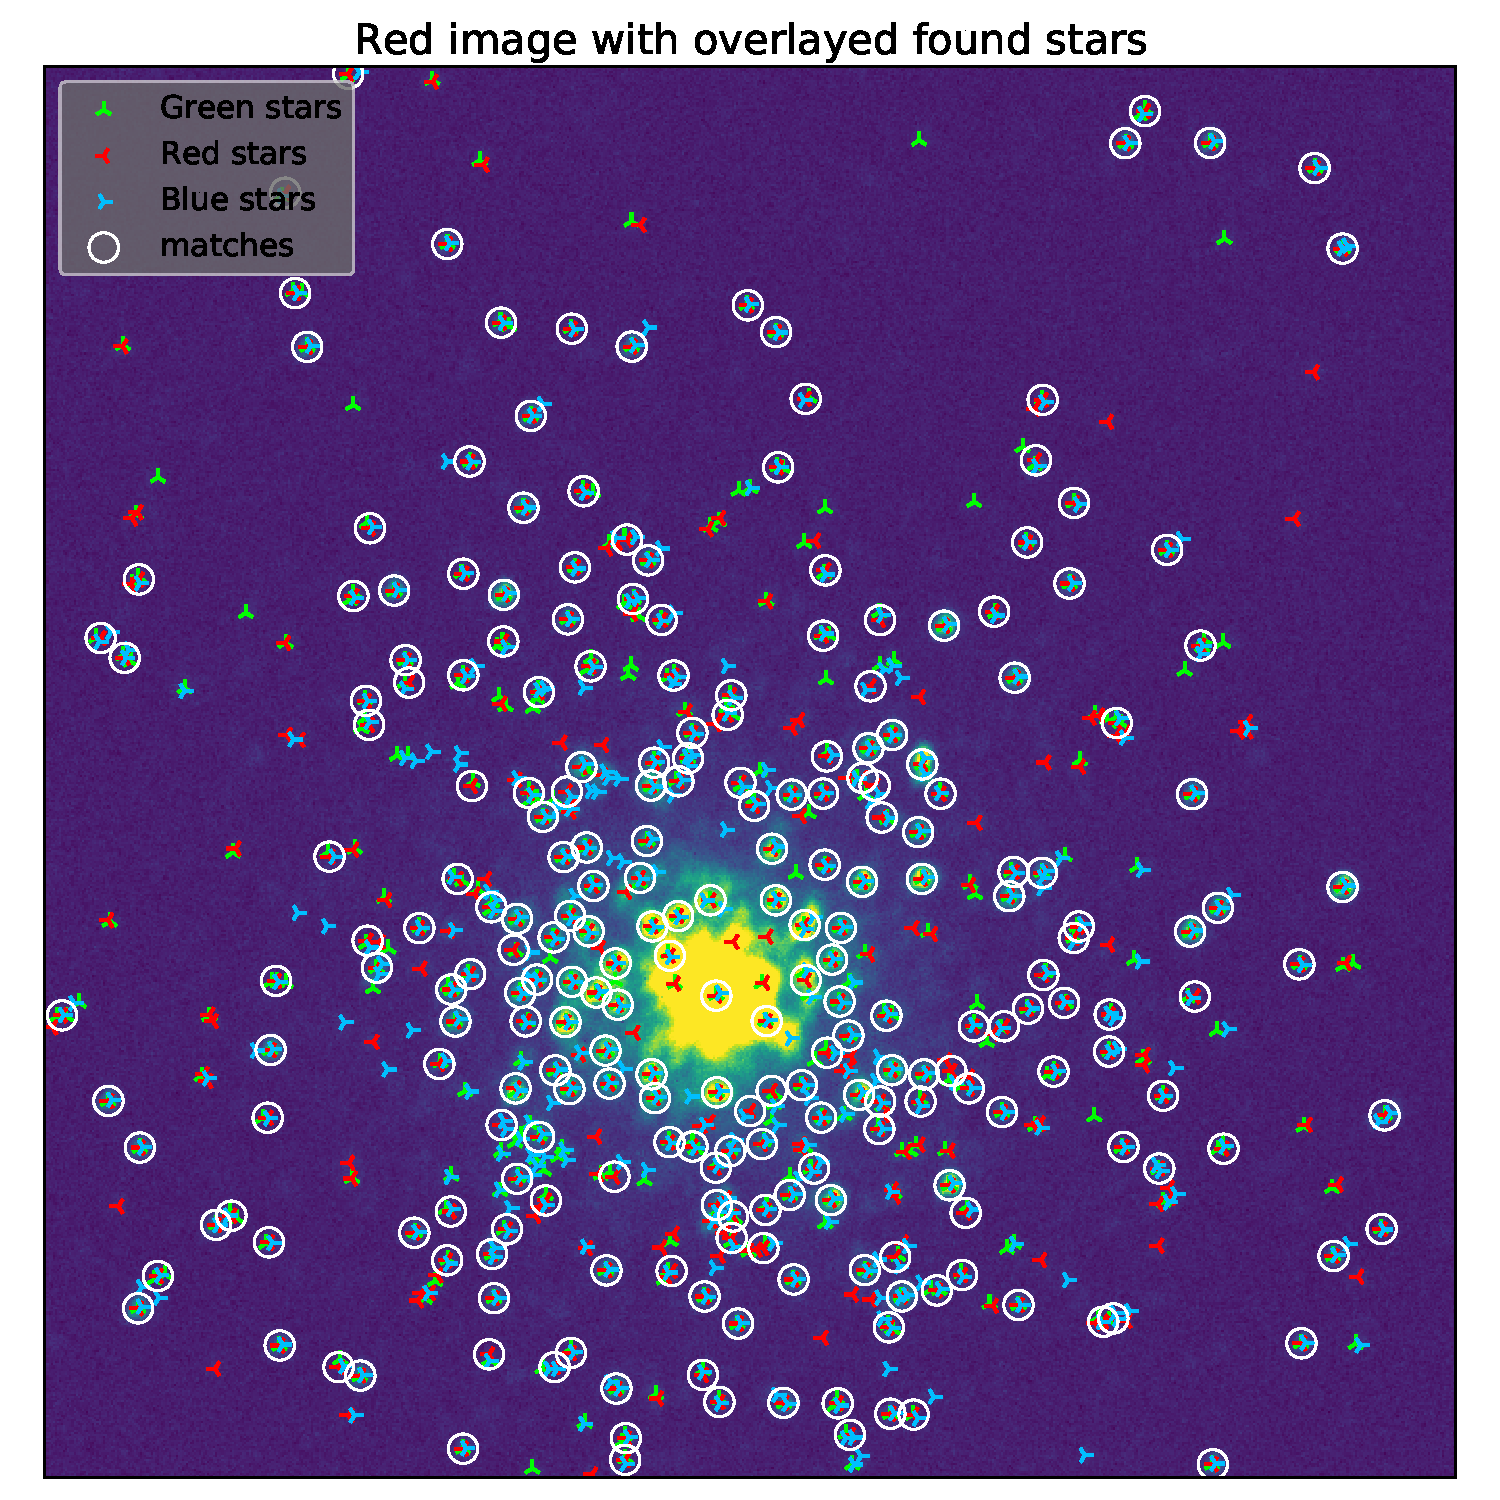
\includegraphics[width=.75\textwidth]{stars.pdf}
\caption{A zoom in of the center of the cluster. Stars outside of this region were also analyzed, but this image is zoomed in for clarity. The white circles are around stars that were found after cross-matching and error-cutting. These stars have arbitrarily low error on their PSF photometry and are in all three colors.}
\label{fig:stars}
\end{figure}


\begin{table}[ht]
\centering
\begin{tabular}{clc}
Step                                             & Color & Number \vspace{1ex}\\ \hline
\multicolumn{1}{r|}{\multirow{3}{*}{Photometry}} & Red   & 927    \\
\multicolumn{1}{r|}{}                            & Green & 913    \\
\multicolumn{1}{r|}{}                            & Blue  & 919    \vspace{2ex}\\
\multicolumn{1}{r|}{\multirow{3}{*}{Error Cut}}  & Red   & 665    \\
\multicolumn{1}{r|}{}                            & Green & 703    \\
\multicolumn{1}{r|}{}                            & Blue  & 633    \vspace{2ex}\\
\multicolumn{1}{r|}{Cross Matched}               & All   & 513    \vspace{2ex}\\
\multicolumn{1}{r|}{\begin{tabular}[r]{@{}r@{}}Cross Matched \\ (Error cut)\end{tabular}} & All & 415
\end{tabular}
\caption{The count of stars at each step of processing. The arbitrary goal set was to keep about half of the stars that was started with, so around 400-500 stars. The pruning ended with about 400 stars, and that was close enough to the goal.}
\label{tab:counts}
\end{table}


\subsection{Calibration}
The final step that needed to be done before creating the CMD was to calibrate it to another survey. For this, the Sloan Digital Sky Survey (SDSS) was used to calculate the average magnitude that each of the filters were off by. Requesting all the stars around M15 with a radius of 0.3 deg returned a total of 256 stars. Doing the same cross-matching of this list against the stars already picked out, a total of 19 matches were found. This is a pretty low number, but still more than enough to calibrate the data. Comparing the filter ranges of the filters used to those of the SDSS survey, it was figured that the closest matches that could be done can be seen in Table~\ref{tab:wavelengths}. Because of a lack of good match for the blue image, the green SDSS data was used for both the blue and green; the range extends over both of them anyways.

\begin{table}[ht]
\centering
\begin{tabular}{llcc}
                             & Filter       & \multicolumn{2}{c}{Range (nm)} \vspace{1ex}\\ \hline
\multirow{3}{*}{Our Filters} & Red          & 600            & 700           \\
                             & Green        & 500            & 600           \\
                             & Blue         & 400            & 500           \\ \hline
\multirow{4}{*}{SDSS Filter} & Infr-red     & 700            & 850           \\
                             & Red          & 500            & 750           \\
                             & Green        & 400            & 500           \\
                             & Ultra-violet & 350            & 400           \\ \hline
\end{tabular}
\caption{The filters used by our data and by the SDSS data that was calibrated against. Both our Red and Green match up best with the SDSS Red and our Blue matches up best with the SDSS Green. The SDSS Ultra-violet was initially used for the calibration, but for the survey pulled the UV light was not defined and has magnitudes several magnitudes brighter than Sol. So, the closest that was viable was the Green. \citep{filter}}
\label{tab:wavelengths}
\end{table}


\section{Results}
\begin{figure}[ht]
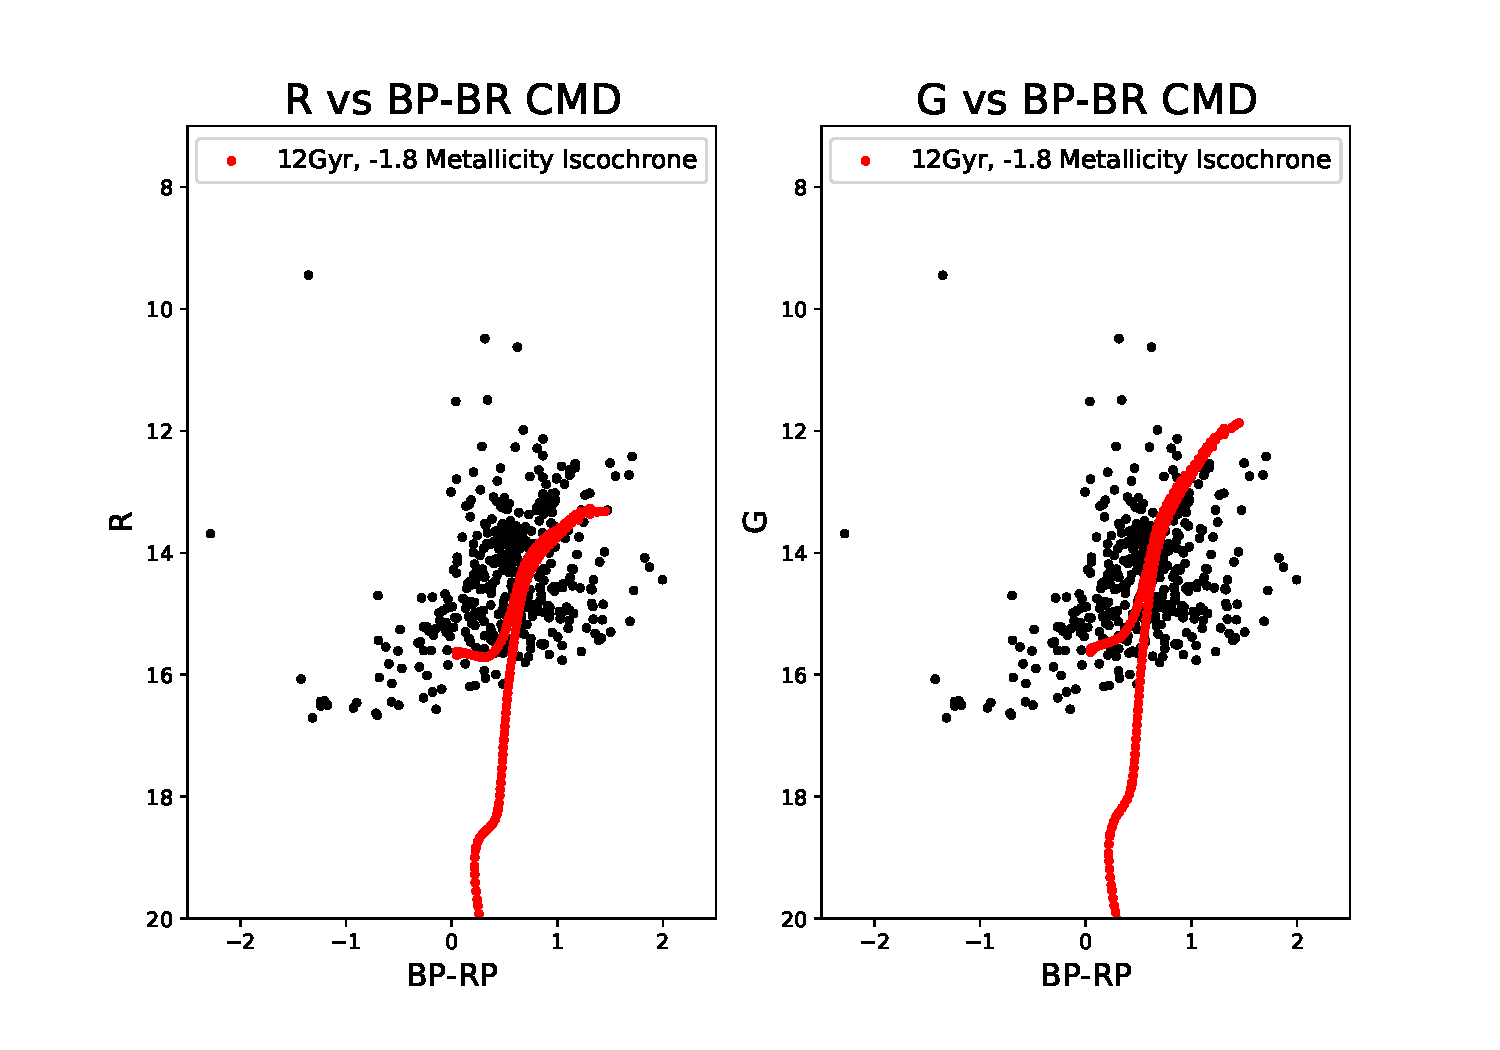
\includegraphics[width=\textwidth]{cmd.pdf}
\caption{The final CMD generated. The isochrones used were given a distance modulus (horizontal shift) of 0 and a extinction coefficient (vertical shift) of 15.1. You can see the characteristics of the horizontal branch and the end of the main branch. The G vs. BP-BR shoes off these characteristics a little better than the R vs. BP-BR plot.}
\label{fig:cmd}
\end{figure}

With the data calibrated, all the image processing and data analysis has been done and the CMD should ready to be made. The usual convention for CMDs is to plot the color along the horizontal axis and the magnitude along the vertical, as can be seen in Figure~\ref{fig:cmd}. The general characteristics here are very hard to see, and the main reason for this is how short the exposure time was. Because of the lack of tracking, to prevent smearing the exposure had to be short. This meant that higher magnitude stars couldn't be seen in the quality images. What can be seen here is a portion of the very prominent horizontal branch that characterizes M15. 

To describe the CMD with theory, the an isochrone model was pulled from [cite the iso one here], and translated to the primary spread of the CMD. This translation reflects primarily unaccounted extinction rates in the data. Since the CMD focuses on such a small section of the star cluster, only the high luminosity characteristics could be pulled out and the lack of a main body meant that it was nearly impossible to accurately characterize the age of the image. For this reason, the age, of 12Gyr, was simply taken from Wikipedia and can be seen to have a moderately decent fit to the scatter plot. 



\section{Discussion and Summary}
Reflecting on the project as a whole, none of the individual steps didn't work. Looking especially at the image processing and data analysis, the information in the image all came out very nicely. The largest error that propegated through the whole generation of the CMD was the lack of experience with the telescope. If was more experience and data was collected on separate occasions, there is no question that the whole body of the CMD would be able to be characterized. It is interesting how the image analysis steps that were taken in this project, while not yielding any boldly insightful results for this project, has developed understanding of the methods used in automatically characterizing visual data from a computationally rigorous approach. \citep{prometheus} \citep{bozepy}


\vskip 0.2in
\bibliography{references}

\end{document}
